\newcommand{\Harmonization}{
  \begin{figure}
    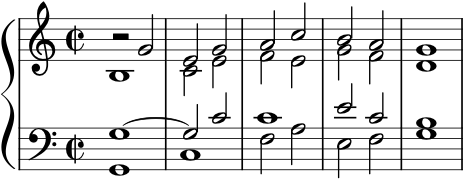
\includegraphics[width=5.5cm]{fig/piston.png}
    \hspace{1cm}
    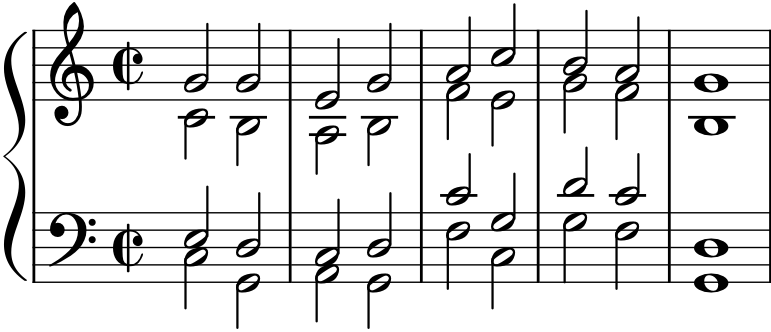
\includegraphics[width=5.5cm]{fig/harmmt.png} \\
    \begin{flushleft}
    \begin{small}
     \hspace{2.1cm} V \ \ \ \ \ \ \ \,I \ \ \ \ \ \ \ \,IV \,VI \ \,III \ IV \ \ \,V
     \hspace{2.65cm} I \ \ V \ \ \ VI \ V \ \ IV \ I \ \ \ V  \,IV \ \ \ \ V
    \end{small}
    \end{flushleft}
    \caption{Harmonization by Piston (left) and Our Implementation (right)}
    \Description{Harmonization by Piston (left) and Our Implementation (right)}
    \label{fig:harmonization}
  \end{figure}
}

\newcommand{\HarmonizationF}{
  \begin{figure}
    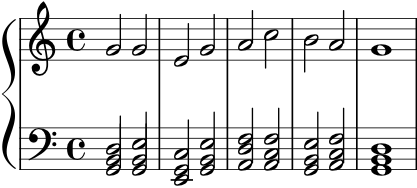
\includegraphics[width=5.5cm]{fig/fharm.png}
    \begin{flushleft}
    \begin{small}
     \hspace{5.5cm} V \,III \ \ \ I \ \,III \ \,II \,IV \ \,III IV \ \ V
    \end{small}
    \end{flushleft}
    \caption{Harmonization by \fharm}
    \Description{Harmonization by \fharm}
    \label{fig:harmonizationF}
  \end{figure}
}

\section{Harmony}
\label{sec:harmony}

Harmony refers to simultaneously sounding tones (chords) and its study
is primarily concerned with the progression of chords throughout a
piece of music. It is in essence the dual of counterpoint. In this
section we formalize a small part of the classic text
\citet{piston-harmony}, in particular part of Chapter~9 which is
concerned with techniques for harmonizing a given melody.
The complete implementation can be found in \texttt{Harmony.agda}
and \texttt{Piston.agda} of the anonymized supplement.

\subsection{Harmonic Progression}
\label{sec:harmony:prog}

The primary Example~9.1 in Piston's text
(Figure~\ref{fig:harmonization} left) shows a
sample four part SATB harmonization in C~major. The melody is the
series of highest notes, i.e., the soprano (S) line, while the other three
parts alto (A), tenor (T), and bass (B) are the melodies below
it. Roman numerals denote the names of the triads at each vertical
slice. Note that even though the example consists of four voices there are only
three distinct pitches sounding at each vertical slice (where tones an
octave apart are considered to have the same relative pitch). As is
typical the root of the triad is always doubled. Also note that all
triads are in root position (i.e., the root is in the bass voice),
as Piston restricts to this case initially in the chapter (he does
relax it later). The goal of a harmonization is both to create an
aesthetically pleasing chord progression as well as fluid melodies in
each voice (called voice leading) and independence of each music
line (in other words good counterpoint). In this chapter
Piston gives advice on how to achieve these goals.

\Harmonization

We would like to formalize some of this advice and apply it to
automate harmonization of melodies. We start with selection of the
sequence of triads, in other words the harmonic progression. Earlier
in the text (on page~23) Piston presents a Table of Usual Root
Progressions, noting which triads usually follow a given one and
which are sometimes used or rare. It is easy to encode this in Agda
using the triad datatype explained in Section~\ref{sec:music}.

\begin{alltt}
record NextTriad : Set where
  constructor nextTriad
  field
    usual : List Triad; sometimes : List Triad; rare : List Triad

rootProgression : Triad \(\rightarrow\) NextTriad
rootProgression I   = nextTriad (IV :: V :: []) (VI :: []) (II  :: III : [])
rootProgression II  = nextTriad (V :: []) (IV :: VI :: []) (I :: III :: [])
rootProgression III = nextTriad (VI :: []) (IV :: []) (I :: II :: V :: [])
rootProgression IV  = nextTriad (V :: []) (I :: II :: []) (III :: VI :: [])
rootProgression V   = nextTriad (I :: []) (IV :: VI :: []) (II :: III :: [])
rootProgression VI  = nextTriad (II :: V :: []) (III :: IV :: []) (I :: [])
rootProgression VII = nextTriad (I  :: III :: []) (VI :: []) (II :: IV  :: V :: [])
\end{alltt}

It is easiest to create a harmonic progression in reverse, to
ensure that one ends a musical phrase with either a full (V--I) or half (V)
cadence, and work backward from there. So we would like to invert this
table to give a list of likely triads to precede a given triad. This
would normally be straightforward but here we see a disadvantage of
using Agda. As is typical with languages based on dependent type
theories, equality is a very subtle concept and even determining if a
term is a member of a list is nontrivial.

In Haskell this would be easy---there is an \texttt{Eq} type class and a
method for automatically generating equalities. In the Agda Standard
Library~\citep{agda-stdlib} list membership is a relation with
constructive evidence of membership, and requires far more effort than we
would like, given that we currently do not need to do
proofs. Alternatives include defining decidable equality for triads
(which requires writing out 49 cases), or mapping to natural numbers
and using already implemented decidable or boolean equality for
those. For now we simply write the inverse function manually,
excluding the rare cases.

\begin{alltt}
previousTriads : Triad \(\rightarrow\) List Triad
previousTriads I   = V :: IV :: VII :: []
previousTriads II  = VI :: IV :: []
previousTriads III = VI :: VII :: []
previousTriads IV  = I :: V :: II :: III :: []
previousTriads V   = I :: IV :: II :: VI :: []
previousTriads VI  = IV :: I :: II :: V :: VII :: []
previousTriads VII = []
\end{alltt}

\subsection{Completing the Harmonization}
\label{sec:harmony:complete}

As Piston does we require the harmonizing triad to include the melody
note. We use a function \texttt{harmonizations} to generate a list of
all candidate harmonizations for a given melody (see
\texttt{Harmony.agda} for its definition). Here again we encounter difficulties
with equality and membership. We use a bit vector to represent the
set of scale degrees in a triad, where each scale degree is mapped to
an element of \texttt{Fin 7}. However we are able to make use of
dependent types in the form of vectors to ensure the length of each
harmonization matches the melody, and continue to use vectors in the
following functions where appropriate.

We next restrict to progressions ending in a half cadence (V) to match
Piston's example. This results in 25
candidate progressions. For each pitch and triad pair we construct a
\texttt{harmonizingChord} in root position with the root doubled. The
function \texttt{voiceChord} spaces the notes nicely. All of this work
is done in the function \texttt{voicedHarmonizations}.

\begin{alltt}
voicedHarmonizations : \{n : N\} \(\rightarrow\) Vec Pitch n \(\rightarrow\) List (Vec (Vec Pitch 4) n)
voicedHarmonizations \{n\} ps =
  let ds = map pitchToDegreeCMajor ps
      hs : List (Vec Triad n)
      hs = filter halfCadence (harmonizations ds)
      in map (\(\lambda\) ts \(\rightarrow\) map (\(\lambda\) pt \(\rightarrow\)
             \(\text{proj}_1\) pt :: harmonizingChord (\(\text{proj}_1\) pt) (\(\text{proj}_2\) pt)) (zip ps ts)) hs
\end{alltt}

To determine the ``best'' of these harmonizations, we now make use of
\texttt{motionCheck} from the counterpoint work. We compare all six
pairs of melodies, count the number of motion errors present, and pick
the harmonization which minimizes these flaws. The function to
determine all errors is straightforward.

\begin{alltt}
motionErrors : \{n : N\} \(\rightarrow\) Vec (Vec Pitch 4) n \(\rightarrow\) List MotionError
motionErrors xs =
  let ss = map (head) xs
      as = map (head \(\circ\) tail) xs
      ts = map (head \(\circ\) tail \(\circ\) tail) xs
      bs = map (head \(\circ\) tail \(\circ\) tail \(\circ\) tail) xs

      sas = map pitchPairToPitchInterval (toList (zip as ss))
      sts = map pitchPairToPitchInterval (toList (zip ts ss))
      sbs = map pitchPairToPitchInterval (toList (zip bs ss))
      ats = map pitchPairToPitchInterval (toList (zip ts as))
      abs = map pitchPairToPitchInterval (toList (zip bs as))
      tbs = map pitchPairToPitchInterval (toList (zip bs ts))
  in concatMap checkMotion (sas :: sts :: sbs :: ats :: abs :: tbs :: [])
\end{alltt}

The harmonization produced is shown in Figure~\ref{fig:harmonization}
right.

\subsection{Comparison with Previous Work}
\label{sec:harmony:compare}

\HarmonizationF

Most of the Haskell-based work on
music~\citep{magalhaes-harmtrace,koops-fharm,magalhaes-fcomp} has
focused on harmony. In particular \fharm~\citep{koops-fharm} tackles
the problem of harmonizing a melody;
Figure~\ref{fig:harmonizationF} shows their harmonization of
Piston's example. Their method is quite different from
ours. Instead of using Piston's table of root progressions they use a
more sophisticated hierarchical grammar from previous
work~\citep{magalhaes-harmtrace}.
More specifically, they first require the melody notes to be members of
the harmonizing chords, then use their previous work to try to create
a harmonic analysis of every possible sequence of chords that arises,
choosing the one that most closely fits their grammar.

Although the result produced by \fharm is not bad, it clearly leaves
room for improvement. Noted in
the paper is that no attention is given to voicing (how each of the
four parts flows horizontally and how the lines interact---in other
words the counterpoint). They use inversions to ensure each melody line
does not move too much, but as the harmonizing triads are all in close
position separated from the melody, the result sounds like a soprano
melody with block chord accompaniment, rather than four independent
lines.

Among those issues not discussed in the paper, one is the choice of
notes to be doubled: \fharm always doubles the melody note, while
in four part harmony it is generally preferred to double the root
note as Piston does.
Another concern is that minimizing the number of parse errors as a means
to choose the best harmonization does not necessarily have a musical
meaning.

Our harmonization follows Piston's rules more closely and has arguably
better spacing of voices; readers can decide for themselves which is
more pleasing.
